\documentclass[conference]{IEEEtran}
%\usepackage{graphics}
\usepackage[skip=-3pt]{caption}
%\usepackage[tableposition=top]{caption}
%\usepackage{caption}
%\captionsetup{font=footnotesize,justification=centering,labelsep=period}
\usepackage{floatrow}
\floatsetup[table]{capposition=top}
\usepackage{graphicx}
\usepackage{multicol}
\usepackage[tight,footnotesize]{subfigure}
%\usepackage[caption=false]{caption}
%\usepackage[font=footnotesize]{subfig}
\usepackage{array}
\usepackage{amsfonts}
%\usepackage{amssymb}
\usepackage{amsmath, amssymb}
\DeclareMathOperator*{\argmax}{argmax}
\usepackage[export]{adjustbox}
%\usepackage{subcaption}
%\usepackage{cite}
%\usepackage{times}
\usepackage{color}
\usepackage{fixltx2e}  
\usepackage{graphicx,tipa}% http://ctan.org/pkg/{graphicx,tipa}
%\usepackage{autoref}
%\usepackage{amsthm}
%\usepackage{algorithmicx}% http://ctan.org/pkg/algorithm
%\usepackage{algpseudocode}% http://ctan.org/pkg/algorithmicx
%\usepackage{algorithm}
\usepackage[ruled,linesnumbered,vlined]{algorithm2e}
\SetAlFnt{\footnotesize}
\SetKw{KwDownTo}{downto}
\SetKw{KwTrue}{true}
\SetKw{KwFalse}{false}
\SetKwInOut{Input}{Input}
\SetKwInOut{Output}{Output}
\SetKw{KwAnd}{and}

\usepackage{algorithmic}
\renewcommand*{\algorithmcfname}{\footnotesize{Algorithm}}
\newcommand{\LineIf}[2]{ \State \algorithmicif\ {#1}\ \algorithmicthen\ {#2} \algorithmicend\ \algorithmicif }
\newcommand{\LINEFOR}[2]{%
    \STATE\algorithmicfor\ {#1}\ \algorithmicdo\ {#2} \algorithmicend\ \algorithmicfor%
}
%%%%%%%%% theorem environment 
\usepackage{amsthm}
\renewcommand{\algorithmicrequire}{\textbf{Input:}}
\renewcommand{\algorithmicensure}{\textbf{Output:}}
\newcommand{\algorithmicbreak}{\textbf{break}}
\newcommand{\BREAK}{\STATE \algorithmicbreak}
\newcommand{\algorithmiccontinue}{\textbf{continue}}
\newcommand{\CONTINUE}{\STATE \algorithmiccontinue}
\renewcommand{\algorithmiccomment}[1]{// #1}
\usepackage{capt-of}
%\usepackage[keeplastbox]{flushend} %to adjust the height of two column at the last page
\newcommand{\subparagraph}{}
\usepackage{titlesec} 
\titlespacing\section{0pt}{3pt plus 0pt minus 2pt}{3pt plus 0pt minus 2pt}
\titlespacing\subsection{0pt}{2pt plus 0pt minus 2pt}{2pt plus 0pt minus 2pt}
\renewcommand{\IEEEQED}{\QEDopen}
%\def\IEEEbibitemsep{0pt plus 0pt}
%\renewcommand{\baselinestretch}{0.98}
%\IEEEilabelindent 0.1in
%\IEEEiednormlabelsep 0.1in
%\IEEEiedtopsep 0in
%\IEEEiedmathlabelsep 0in
%\setlength{\abovedisplayskip}{0pt plus0pt minus4pt}%
%\setlength{\belowdisplayskip}{\abovedisplayskip}%
%\setlength{\abovedisplayshortskip}{0pt plus0pt}%
%\setlength{\belowdisplayshortskip}{0pt plus0pt minus4pt}
\setlength{\abovecaptionskip}{0ex}
\setlength{\belowcaptionskip}{0ex}
%\setlength\floatsep{0pt plus 0pt minus 0pt} % define the vertical space two adjacent floats
%\setlength\textfloatsep{5pt plus 2pt minus 0pt} % for floats on top and bottom of text only; For floats at top - length between float and text below it. For floats at bottom - length between float and text above it
%\setlength\intextsep{0pt plus 0pt minus 0pt} %  for floats in the middle of text only - length between text above it, and text below it.
\begin{document}
%
% paper title
% can use linebreaks \\ within to get better formatting as desired
%\title{Hole Bypassing Geographic Routing Protocol with Delay Guarantee in WSNs}
%A Delay Delay Guaranteed Geographic Routing Protocol with Hole Avoidance in WSNs
%\title{A Geographic Routing Protocol with Delay Guarantee and Hole Avoidance for WSNs} 
\title{Deep Convolutional LSTM Network-based Traffic Matrix Prediction with Partial Information} 
%Hole Avoidance Geographic Routing Protocol with 
%Geographic Routing with Delay Guarantee and Hole Avoidance in WSNs} 
% author names and affiliations
% use a multiple column layout for up to three different
% affiliations
\author{ \IEEEauthorblockN{Van An Le\IEEEauthorrefmark{1}, Phi Le Nguyen\IEEEauthorrefmark{1}, Yusheng Ji\IEEEauthorrefmark{1}\IEEEauthorrefmark{2},}
    \IEEEauthorblockA{\IEEEauthorrefmark{1}Department of Informatics, SOKENDAI (The Graduate University for Advanced Studies), Tokyo, Japan} 
    \IEEEauthorblockA{\IEEEauthorrefmark{2}National Institute of Informatics, Tokyo, Japan} 
    \IEEEauthorblockA{Email: \IEEEauthorrefmark{1}\{anle, nguyenle, kei\}@nii.ac.jp}
}
% make the title area
\maketitle
\begin{abstract}
Accurate prediction of the future network traffic plays an important role in various network problems (e.g. traffic engineering, capacity planning, quality of service provisioning, etc.). However, the modern network communication is extremely complicated and dynamic, which makes the tasks of modeling and predicting the network behavior very difficult. 
%Moreover, although the prediction accuracy largely depends on the amount of historical data, measuring all the network traffic is impossible or impractical due to the monitoring resources constraints as well as the dynamics of temporal/spatial fluctuations of the traffic. 
To this end, a common approach is to apply the traditional time series prediction techniques such as Autoregressive Integrated Moving Average or Linear Regression. 
Besides that, there are some studies exploiting Deep Learning techniques such as Restricted Boltzmann Machine or Recurrent Neural Network (RNN) to estimate the traffic volume. 
%Unfortunately, all of the existing algorithms require precise historical data as the input. However, measuring all the network traffic is impossible or impractical due to the monitoring resources constraints as well as the dynamics of temporal/spatial fluctuations of the traffic.  
Although the prediction accuracy largely depends on the amount of historical data, measuring all the network traffic is impossible or impractical due to the monitoring resources constraints as well as the dynamics of temporal/spatial fluctuations of the traffic. Thus, the state-of-the-art proposals reveal poor performance regarding the traffic inference when lacking ground-truth input.

In this paper, we propose a highly accurate traffic prediction algorithm by leveraging the Convolutional LSTM network (ConvLSTM), which is the integrated model of Convolutional Neural Network (CNN) and Long Short-Term Memory (LSTM) network, for spatiotemporal modeling and estimating the future network traffic. We also propose a technique which exploits the RNN to correct the imprecise data in the input. 
To evaluate the proposed algorithm, we conduct extensive experiments using the Abilene dataset which contains the real network traffic trace. The experiment results show that our proposed approach outperforms the existing algorithms in terms of several metrics including error ratio, root mean square error, and coefficient of determination, in both one-step-ahead and multi-step-ahead prediction with partial information.
%can achieve significantly better prediction accuracy in terms of several metrics including error ratio, root mean square error, and coefficient of determination in both one-step-ahead and multi-step-ahead prediction under the extreme condition of missing ground-truth input.

\end{abstract}
%%%%%%%%%%%%%%%%%%%
\newtheorem{mydef}{Definition}
\newtheorem{mylemma}{Lemma}
\newtheorem{mytheorem}{Theorem}
\newtheorem{myalgo}{Algorithm}
\newtheorem*{myproof}{Proof}
\newtheorem{myproposition}{Proposition}
\newtheorem{mycon}{Condition}

\section{Introduction}
\label{sec:introduction}
In recent years, the great demand for the Internet services (e.g. video streaming, VoIP, etc.) has led to an exponential growth in the backbone network traffic. 
Having a better knowledge about the backbone network traffic, specifically being able in predicting future traffic, thus becomes a critically important factor to perform management tasks such as traffic engineering, capacity planning and quality of service provisioning. 
For example, in the well-known Network Utility Maximization (NUM) \cite{xu2018experience}, \cite{low1999optimization} (which usually provides a bandwidth allocation or smart routing solution by solving optimization problem), the future network traffic knowledge (e.g. user demands, link usages, end-to-end latency) is used as the input. 
%These important factors are usually in the form of a traffic matrix (TM), which represents the traffic volume or latency between the origins (i.e. sources) and destinations in the network. 
However, due to the explosion of backbone network traffic as well as the complexity and dynamics of network communication behavior, modeling and estimating the future traffic in backbone networks becomes a significant challenge.

In the literature, numerous effort has been done on predicting future traffic in data centers and cellular networks.
In the traditional approaches, regression techniques (e.g., Autoregressive Integrated Moving Average (ARIMA) \cite{box2015time}) are exploited to obtain the predicted value. However, ARIMA has shown a poor performance due to two main reasons: 1) The communication behavior has become too dynamic and complicated to be modeled by a linear system. 2) ARIMA ignores the spatial relation between the traffic flows and processes the flows independently. However, the recent studies have shown that there is a strong relation between the flows, which can be utilized to improve the prediction accuracy \cite{wang2017spatiotemporal}, \cite{xie2016accurate}. 
Recently, deep learning has been widely applied to various application domains such as image/video processing, natural language recognition, etc., and achieved breakthrough results. 
In traffic analysis domain, deep learning algorithms have shown superior capability in solving the modeling and predicting non-linear time series problems. Nie et al. \cite{nie2016traffic} used Restricted Boltzmann Machine to accurately predict the future traffic volume.
Alternatively, the studies in \cite{wang2017spatiotemporal} and \cite{cao2018interactive} exploited the Convolutional Neural Network (CNN) and Long Short-Term Memory (LSTM) for capturing the spatial and temporal features. 

Unfortunately, all of the existing algorithms proposed so far require precise historical data as the input.
This requirement can be easily accomplished in the context of data centers and cellular networks since these networks are controlled through top-of-rack switches or base stations, respectively. 
However, collecting all the traffic data in backbone networks is impractical due to the complexity of network topology, the resource limitation of network devices and the high overhead of monitoring high-speed network. 
Therefore, estimating the future traffic in backbone networks suffers from the problem of missing ground-truth input where some traffic flows cannot be monitored at a particular time. 
A common approach to fill into the missing data is utilizing the data generated by the prediction model.
However, this may cause a huge degradation in the prediction's performance. 

In this paper, we address the problem of modeling and predicting the future traffic in backbone networks under the lack of historical traffic data. 
More specifically, we focus on predicting the future traffic matrices which represent the traffic volume between all the origins (i.e., sources) and the destinations in the network. 
We leverage the so-called Convolutional LSTM  (ConvLSTM, for short) network \cite{xingjian2015convolutional} (i.e., a combination of CNN and LSTM network) in extracting and modeling the spatiotemporal feature of the traffic matrix data. 
Besides that, since the prediction accuracy of the model strongly depends on the preciseness of feeding data, the most challenging problem is how to correct the feeding data so as to minimize the gap between the feeding data and the ground-truth. 
To this end, we propose two techniques. First, by constructing a backward network which processes the input in the inverse order of time, we have more information to correct the previous predicted data (which is usually imprecise) before feeding it into the model to predict the future traffic. Secondly, we construct a mechanism to sample the ground-truth at a certain rate. Specifically, by comparing the trend and the error in the historical prediction of each flow, we design a formula to determine which flows should be monitored at the next timestep. By doing so, we can balance between the monitoring overhead (in terms of flow monitoring rate) and the prediction accuracy. 
The contribution of this paper can be summarized as follows:
\begin{itemize}
\item To our best knowledge, we are the first one considering the problem of predicting future traffic in backbone networks where the historical data may be missed. Our approach is different from existing deep learning approaches in time series prediction where the model is fed with only the ground-truth input.
\item We exploit the ConvLSTM in handling the spatiotemporal of the traffic matrices in backbone networks and construct a model which combines the forward and backward ConvLSTM networks. This model is able to correct the input data to improve the accuracy of the future traffic prediction. Moreover, we also design a formula to determine which flows should be measured in the future.
\item We evaluate the performance of our proposed algorithms by conducting extensive experiments on real backbone network traffic dataset and comparing the results with state-of-the-art approaches.
\end{itemize}
The rest of the paper is organized as follows: we first introduce the problem of traffic prediction under the lack of precise input data and give a brief introduction about LSTM and ConvLSTM network in Section 2. Section 3 presents the motivation and the details of our proposed algorithms for correcting the input data and determining the monitored flow set. Section 4 shows extensive experimental results. We present some related works in Section 5 and conclude the paper in Section 6.
% \begin{figure} [bt]
% \centering
% 	\subfigure[Local minimum problem.\label{fig:intro_1}]{
% 	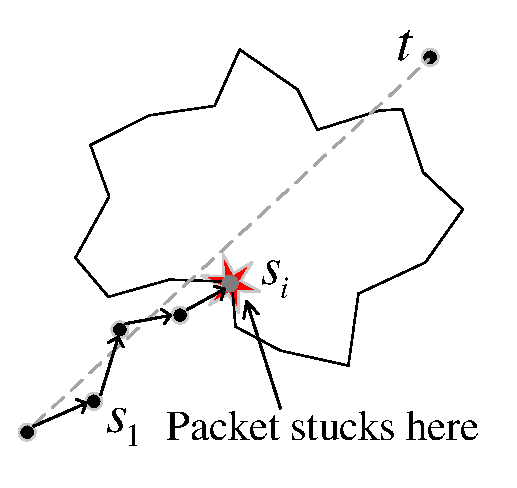
\includegraphics[width=0.35\columnwidth]{./intro_figs/intro_1.eps}
% 	}
% 	\hfill
% 	\subfigure[Congestion around the hole boundary.\label{fig:intro_2}]{
% 	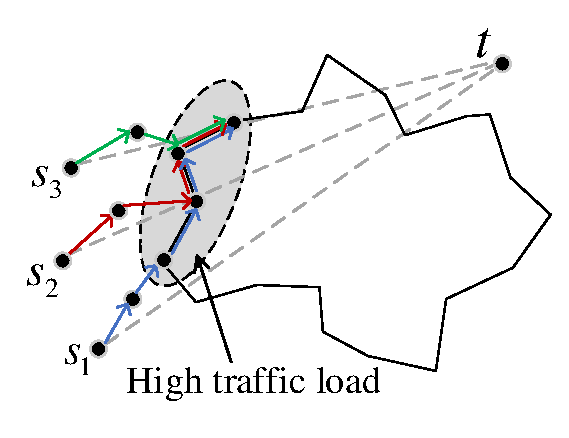
\includegraphics[width=0.4\columnwidth]{./intro_figs/intro_2.eps}
% 	}
% 	\caption{Illustrations of two serious problems that the existing protocols may encounter.}
% 	\label{fig:intro}
% \end{figure}
%
%\begin{figure*}[bt]
%    \centering
%    \begin{subfigure}[t]{0.45\textwidth}
%        \centering
%        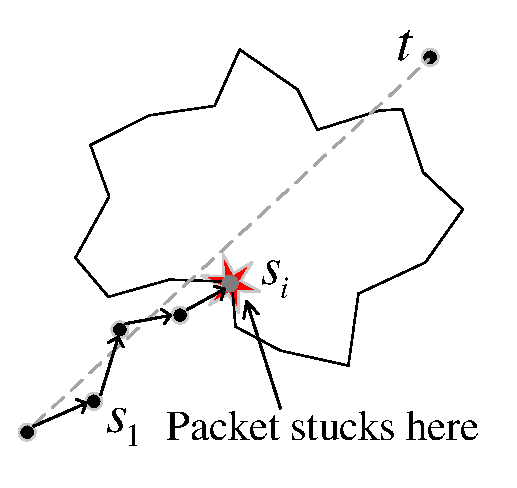
\includegraphics[width=1\columnwidth]{./intro_figs/intro_1.eps}
%        \caption{Local minimum phenomenon where the packets are stopped at the hole boundary.}
%    \end{subfigure}
%    \begin{subfigure}[t]{0.45\textwidth}
%        \centering
%        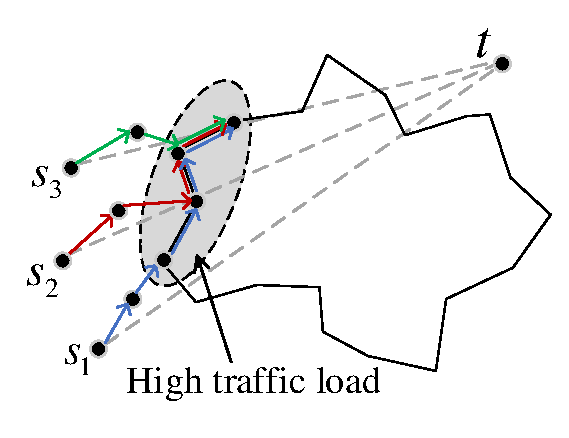
\includegraphics[width=1\columnwidth]{./intro_figs/intro_2.eps}
%        \caption{The nodes surrounding the hole boundary are imposed a heavy traffic load.}
%    \end{subfigure}
%    \caption{Illustration of two serious problems that the existing protocols may encounter.}
%\end{figure*}



\section{Preliminaries}
\label{sec:preliminaries}
In this section, we first present the problem formulation of traffic matrix prediction under the lack of ground-truth input. 
Then, we give a brief introduction about the Long Short-Term Memory and Convolutional LSTM networks which are used in our approach. 
% We summarize the major notations in the table \ref{table:notations} for quick reference.
% \begin{table}[]
% \begin{tabular}{|c|l|}
% \hline
% Notations           & Description                                                                                                                                                              \\ \hline
% N                   & Set of node in the network. |N| = n.                                                                                                                                     \\ \hline
% X                   & The traffic matrix at timestep j                                                                                                                                         \\ \hline
% X$\sim$             & The predicted traffic matrix for timestep j                                                                                                                              \\ \hline
% x                   & Traffic volume of flow (s,d) at timesteps j. x \textbackslash{}in X                                                                                                      \\ \hline
% o                   & The ground-truth value of traffic volume of flow (s,d) at timestep j                                                                                                     \\ \hline
% x$\sim$             & The predicted traffic volume of flow (s,d) for timestep j.                                                                                                               \\ \hline
% x\textasciicircum{} & The predicted traffic volume of flow (s,d) for timestep j by backward network.                                                                                           \\ \hline
% m                   & \begin{tabular}[c]{@{}l@{}}The binary variable, m = 1 indicates that the traffic volume of flow\\  (s,d) at timestep j is ground-truth value and otherwise.\end{tabular} \\ \hline
% M                   & The measurement matrix at timestep j.                                                                                                                                    \\ \hline
% lf                  & The forward loss                                                                                                                                                         \\ \hline
% lb                  & The backward loss                                                                                                                                                        \\ \hline
% w                   & The weight of flow (s,d) is calculated at current timestep t.                                                                                                            \\ \hline
% \end{tabular}
% \caption{My caption}
% \label{my-label}
% \end{table}
\subsection{Problem Description}
\label{subsec:problem_description}
\begin{figure}
\centering
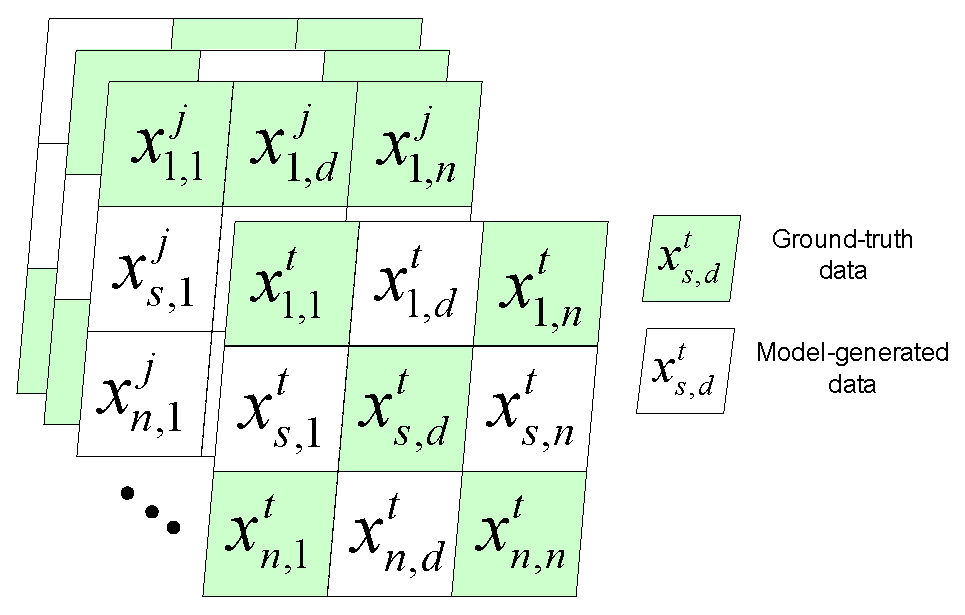
\includegraphics[width=0.6\columnwidth]{preliminaries_figs/traffic_matrices.eps}
		\caption{A sequence of $J$ previous traffic matrices including both ground-truth and imprecise data. \label{fig:traffic_matrices}}
\end{figure}
%\vskip -5ex
%\vspace{-10pt}
%In this section, we present the problem formulation of traffic prediction under the lack of precise input traffic data. 
We suppose that the traffic monitoring and predicting tasks are executed periodically in every \textit{timestep} and denote $t$ as the current timestep. Given a backbone network in which $\mathcal{N}$ is the set of nodes ($\left |  \mathcal{N} \right |=n$), let $X_j \in \mathbb{R}^{n \times n}$ be the traffic matrix at the timestep $j$. Each element $x_{s,d}^j \in X_j$  represents the traffic volume of a flow from a source $s$ to a destination $d$ in the network (flow ($s,d$), for short) at timestep $j$. Thus, the traffic matrix prediction problem is to estimate the traffic matrices of next $L$ timesteps (denoted by $\widetilde{X}_{t+1},...,\widetilde{X}_{t+L}$), given the previous $J$ measurements ($L,J \geq 1$):
\begin{equation}
\begin{aligned}
&\widetilde{X}_{t+1},...,\widetilde{X}_{t+L} \\
	&\quad = \argmax_{X_{t+1},...,X_{t+L}} p(X_{t+1},...,X_{t+L} | X_{t-J+1},...,X_{t})
\end{aligned}
\end{equation}
However, in this paper, we consider the case of backbone networks where we cannot obtain all the $J$ previous traffic matrices by directly monitoring all the flows. Although in recent years, advance network architectures such as Software-Defined Networking (SDN) \cite{mckeown2008openflow} and Network Function Virtualization (NFV) have enabled many alternative ways to measure the network flow information, collecting all the traffic statistics with low overhead (in terms of computational complexity, bandwidth, ...) still remains as a challenging task. Therefore, to reduce the monitoring overhead, we measure only a part of the traffic flows at each timestep and use the data generated by the prediction model to fill into the missed historical data.
%traffic matrix. 
Accordingly, the traffic matrix prediction problem under highly missing ground-truth data can be formulated as follows:

\textbf{Input}
\begin{equation}
\label{equation:tm_prediction_missing_data}
\begin{matrix}
x_{s,d}^{j}=\left\{\begin{matrix}
o_{s,d}^j & \text{if} \ m_{s,d}^j=1 \\
\widetilde{x}_{s,d}^j & \text{otherwise}
\end{matrix}\right. \\

\forall s, d \in N; j = t - J + 1,...,t 
\end{matrix}
\end{equation}

\textbf{Output}
\begin{equation}
\begin{aligned}
\widetilde{X}_{t+1}&,...,\widetilde{X}_{t+L} \\
	& = \argmax_{X_{t+1},...,X_{t+L}} p(X_{t+1},...,X_{t+L} |  X_{t-J+1},...,X_{t})
\end{aligned}
%\end{matrix}
\end{equation} 
where $o_{s,d}^j$ and $\widetilde{x}_{s,d}^j$ denote the observed and predicted value of flow ($s,d$) at timestep $j$, respectively. The binary variable $m_{s,d}^j$ depends on the monitoring policy, where $m_{s,d}^j = 1$ indicates that flow ($s,d$) is monitored at timestep $j$; otherwise, the value of traffic volume is filled up by the prediction result. Fig.\ref{fig:traffic_matrices} shows the sequence of $J$ previous traffic matrices which is used as the input for predicting the future traffic. The green elements are the ground-truth data obtained by monitoring the flows directly, and the white elements represent the predicted values.  
\subsection{LSTM and Convolutional LSTM network for spatiotemporal sequence modeling}
\label{subsection:lstm_ConvLSTM}
\begin{figure}		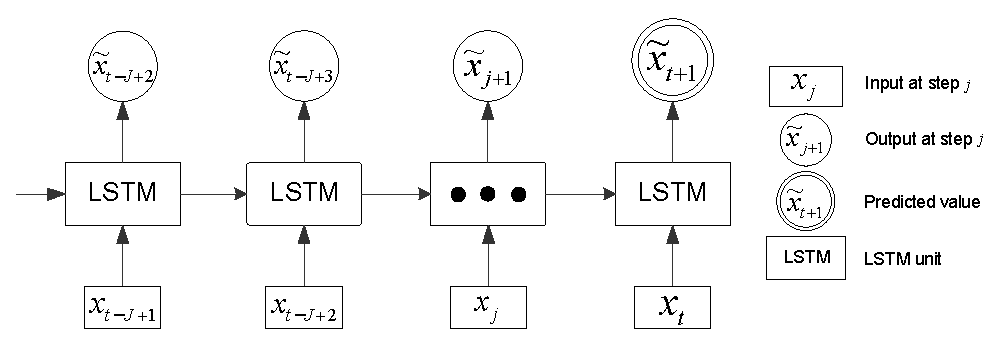
\includegraphics[width=0.8\columnwidth]{preliminaries_figs/LSTM_model.eps}
		\caption{The unfolded model of the LSTM network. \label{fig:LSTM_model}}
        %\vspace{-5pt}
\end{figure}
% \begin{figure}
% \centering
% 		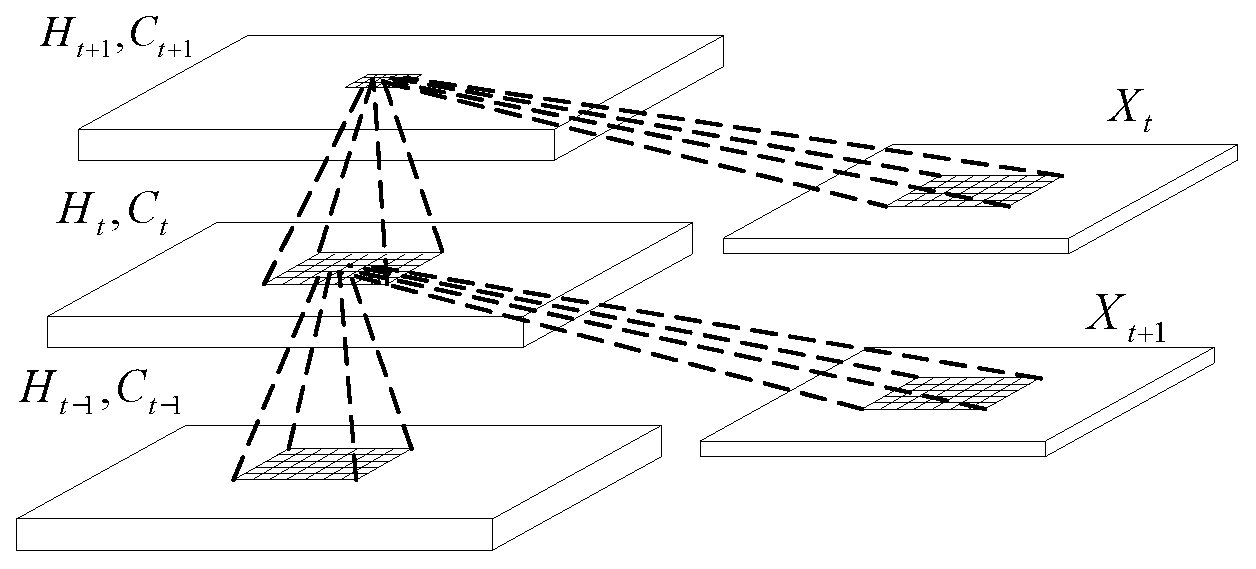
\includegraphics[width=0.65\columnwidth]{preliminaries_figs/ConvLSTM_model.eps}
% 		\caption{The inner structure of ConvLSTM network \cite{xingjian2015convolutional}. 
%         \label{fig:ConvLSTM_model}}
%         \vspace{-5pt}
% \end{figure}
Long Short-Term Memory network is a special Recurrent Neural Network which replaces the standard RNN units by the LSTM units. 
LSTM network has been proved to be stable and powerful for modeling long-range dependencies in various problem domains, thus it is well-suited for processing and making predictions based on time series or sequence data.
Indeed, LSTM has been applied in many real-life sequence modeling problems. 
The unfolded model of LSTM network (Fig.\ref{fig:LSTM_model}) shows that the input is processed step-by-step and the outputs of previous steps are used as the input for the next step. This architecture along with the advantages of the memory cell in LSTM units make LSTM network especially suitable for solving the series based predictions.

However, in many problems such as precipitation nowcasting \cite{xingjian2015convolutional} or images/videos based action prediction where the sequence data has a strong spatial relation, LSTM reveals many limitations. Therefore, to deal with more general spatiotemporal sequence forecasting problems, authors in \cite{xingjian2015convolutional} have proposed an extension of LSTM called ConvLSTM. The ConvLSTM layer has convolutional structures in both the input-to-state and state-to-state transitions which can exploit both temporal and spatial features of the input sequence. To obtain the spatiotemporal feature, the ConvLSTM network takes a 3D tensor $X_t$ as input in the processing step $t$, for example, $X_t$ can be a $32 \times 32 \times 3$ image whose the last dimension represents the color of the image (RGB). The key equations of the ConvLSTM are shown in (\ref{equation:convlstm}), where $i_t, f_t, o_t$ are the input, forget, output gates, respectively; $C_t, H_t$ are the cell and the final state of the LSTM unit, respectively; `$*$' denotes the convolution operator and `$\circ$' denotes the Hadamard product \cite{xingjian2015convolutional}:
\begin{equation}
\label{equation:convlstm}
\begin{aligned}
i_t &= \sigma(W_{xi}*X_t + W_{hi}*H_{t-1} + W_{ci}\circ C_{t-1} + b_i) \\
f_t &= \sigma(W_{xf}*X_t + W_{hf}*H_{t-1} + W_{cf}\circ C_{t-1} + b_f) \\
C_t &= f_t\circ C_{t-1} + i_t\circ \tanh(W_{xc}*X_t + W_{hc}*H_{t-1} + b_c) \\
o_t &= \sigma(W_{xo}*X_t + W_{ho}*H_{t-1} + W_{co}\circ C_{t} + b_o) \\
H_t &= o_t \circ \tanh(C_t)
\end{aligned}
\end{equation}
The main difference between the LSTM unit and ConvLSTM unit is the convolution operation (i.e., `$*$'). While the LSTM network only takes a 1D array as the input at each processing step, the ConvLSTM takes a 3D tensor as the input and uses multiple filters to extract the spatial information. The filter size (also called as kernel size) is $k \times k \times d$, where $k$ is an integer number (normally, $k=3,5,7,etc.$) and $d$ equals to the last dimension of the input. These filters are shifted across the 3D input, and hence, can extract the spatial features of the data.

\section{Proposed Prediction Model}
\label{sec:proposed_prediction_model}
In this section, we first describe two challenges in solving the traffic matrix prediction problem with partial information in Section \ref{subsection:motivation}. 
%under highly missing ground-truth data in Section \ref{subsection:motivation}. 
These two challenges then are addressed in Section \ref{subsection:data_correction} and \ref{subsection:flows_selection}, respectively.
\subsection{Motivation}
\label{subsection:motivation}
\begin{figure}
  \subfigure[10$\%$ Ground-truth input. \label{fig:lstm_prediction_10}]{
  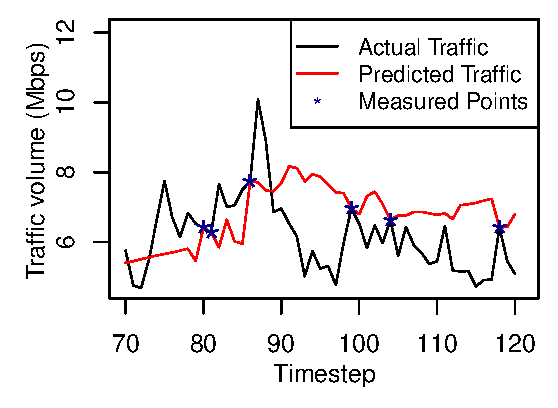
\includegraphics[width=.44\textwidth]{proposed_model_figs/lstm_flow_142_day_10_10.eps}
  }
  \subfigure[20$\%$ Ground-truth input.\label{fig:lstm_prediction_20}]{
  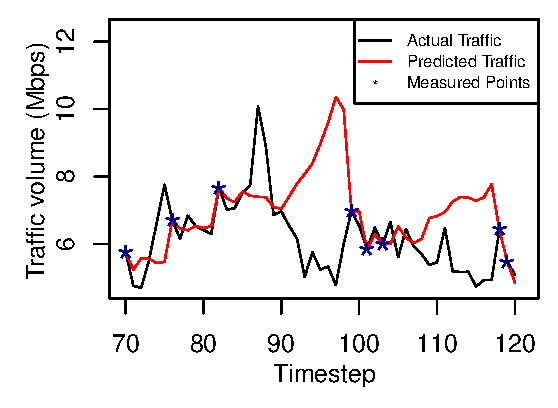
\includegraphics[width=.44\textwidth]{proposed_model_figs/lstm_flow_142_day_10_20.eps}
  }
  \subfigure[30$\%$ Ground-truth input.\label{fig:lstm_prediction_30}]{
  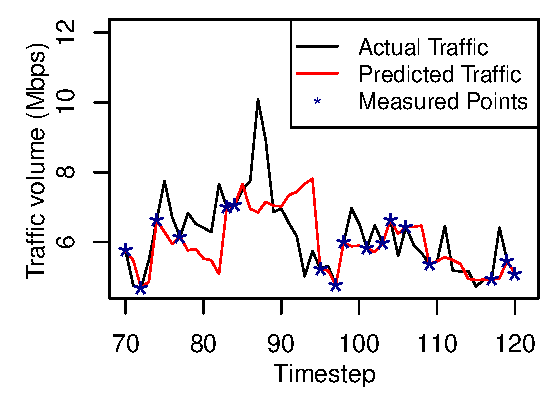
\includegraphics[width=.44\textwidth]{proposed_model_figs/lstm_flow_142_day_10_30.eps}
  }
  \subfigure[40$\%$ Ground-truth input.\label{fig:lstm_prediction_40}]{
  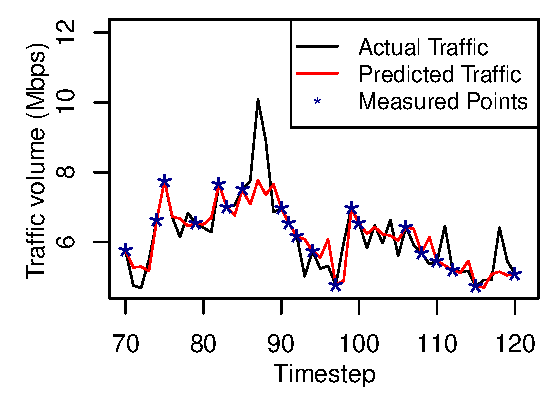
\includegraphics[width=.44\textwidth]{proposed_model_figs/lstm_flow_142_day_10_40.eps}
  }
\caption{The effect of ground-truth input on prediction accuracy. (One-step-ahead prediction using the LSTM network.)}
\label{fig:effect_ground_truth_input}
\vspace{-5pt}
\end{figure}
In order to deploy the traffic matrix prediction model, we face two important challenges. The first one is the accumulative error in the prediction results over timesteps. We have conducted an experiment to figure out the impact of imprecise input data on the results of one-step-ahead prediction (i.e., $L=1$) using the LSTM network. 
%Fig.\ref{fig:semi_recursive_pred_exp} shows the comparison between the ground-truth value and the traffic prediction results which use both precise data (obtained by direct measuring) and imprecise data (the predicted results of previous timesteps). 
Fig.\ref{fig:effect_ground_truth_input} shows the one-step-ahead prediction results with various settings of the percentage of ground-truth data in the input. As shown, the accuracy decreases over the timesteps between two consecutive measurement points (i.e., Fig.\ref{fig:lstm_prediction_10}, Fig.\ref{fig:lstm_prediction_20}). While in Fig.\ref{fig:lstm_prediction_40}, thanks to the higher percentage of ground-truth data in the input, we can capture the trend of the flow and achieve a high accuracy in forecasting the future traffic. Therefore, in order to alleviate the accumulative error while remaining the low monitoring overhead (which is proportional to the portion of the ground-truth data), our idea is to add a preprocessing on the imprecise data before feeding it into the prediction model. Specifically, we propose a novel deep learning model based on the bidirectional recurrent neural network (the details will be shown in Section \ref{subsection:data_correction}).

The second challenge is how to determine which flows to be measured at the next timestep. As mentioned above, in order to reduce the monitoring overhead we do not measure all network flows, thus choosing appropriate flows to monitor in each timestep becomes a critical factor in reducing the prediction error. One of the common approaches in choosing monitored flow set is to satisfy the fairness among all the flows. Specifically, the gaps between every two consecutive monitored timesteps of every flow are kept to be approximately the same. However, this method may not be effective since the network flows are dynamic and have various temporal fluctuation patterns. To deal with this problem, we propose a novel scheme for selecting the next monitored flows, which exploits the previous prediction results and the fluctuation characteristic of all flows (see the details in Section \ref{subsection:flows_selection}).
\subsection{Spatiotemporal traffic matrix prediction and input data correction}
\label{subsection:data_correction}
The ConvLSTM network has shown the effective capability in processing the spatial and temporal time series data where the inputs are 3D tensors such as images or video frames. 
Therefore, to apply the ConvLSTM network in our problem, we first consider the traffic matrices as 2D images with the dimension of $n \times n$, and then we transform them into 3D tensors by adding extra binary matrices (called as measurement matrices). Specifically, the measurement matrix $M_j$, which is added to the traffic matrix at timestep $j$, is a matrix whose each element $m^j_{s,d} \in M_j$ indicates whether the corresponding value in the traffic matrix is an observed value (i.e., $m^j_{s,d}=1$) or a predicted value (i.e., $m^j_{s,d}=0$). 
%Therefore, to apply the ConvLSTM network in our problem, first we consider the traffic matrices as 2D images with the dimension of $n \times n$. Then, we transform these traffic matrices to 3D tensors by adding a binary matrix $M_j$ into the traffic matrix of each timestep $j$. Specifically, $M_j$ is the measurement matrix whose each element $m^j_{s,d} \in M_j$ indicates that the corresponding value in the traffic matrix is an observed (i.e., $m^j_{s,d}=1$) or predicted value (i.e., $m^j_{s,d}=0$). Thus, we have the input of the ConvLSTM network which is a sequence of $J$ 3D tensors with the dimension of $n \times n \times 2$. 
\begin{figure}
\centering	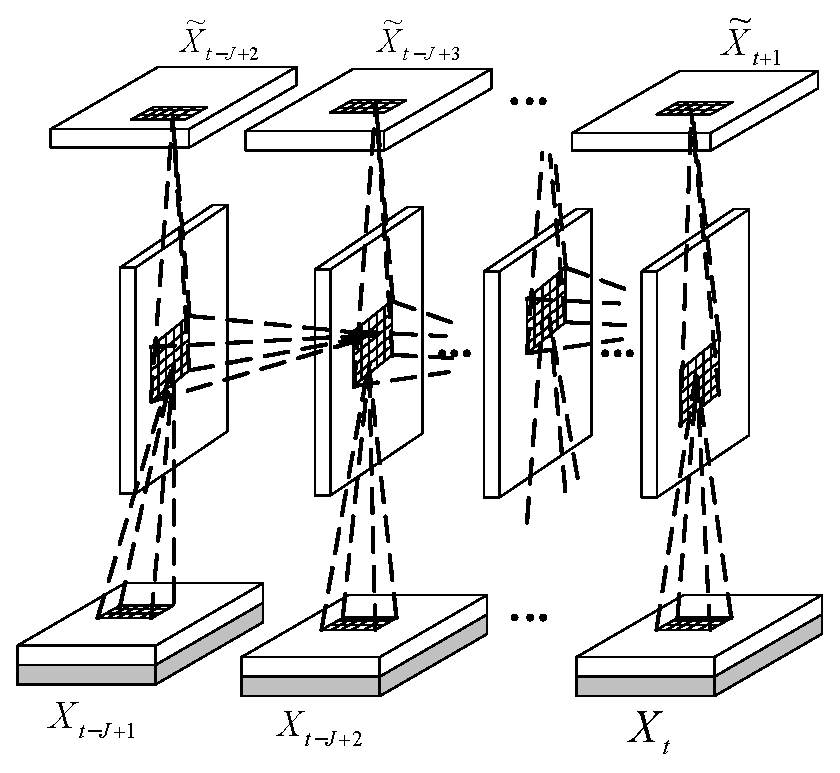
\includegraphics[width=0.6\columnwidth]{proposed_model_figs/ConvLSTM_TM_prediction.eps}
		\caption{The many-to-many model of ConvLSTM network for traffic matrix prediction. \label{fig:ConvLSTM_TM_prediction}}
        \vspace{-5pt}
\end{figure}
Thus, the input of our ConvLSTM network is a sequence of $J$ 3D tensors whose dimension is $n \times n \times 2$. 
In order to predict multi-step traffic matrices, we apply the Iterated Multi-Step estimation (IMS) approach \cite{shi2018machine}. Specifically, we first use the many-to-many model to predict the traffic matrix of the next timestep and then, iteratively feed the generated data into the model to get the multi-step-ahead prediction. Fig.\ref{fig:ConvLSTM_TM_prediction} describes the many-to-many model which takes $J$ 3D tensors from timestep $t-J+1$ to $t$ as the input and predicts the next traffic matrix $\widetilde{X}_{t+1}$. 
\begin{figure*}[bt]
\centering
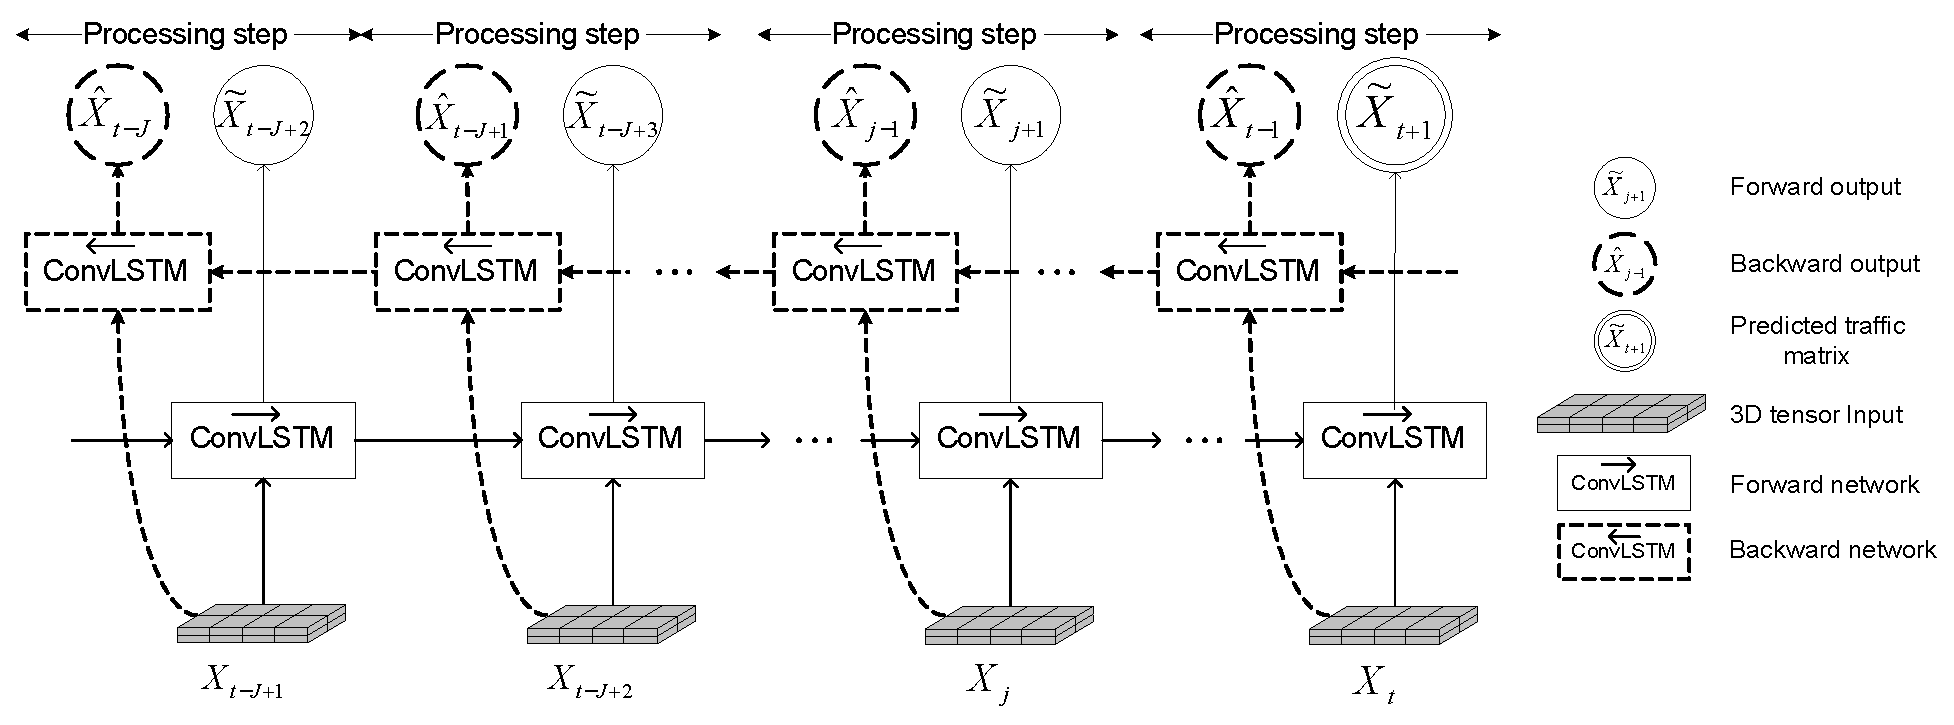
\includegraphics[width=0.65\columnwidth]{proposed_model_figs/forward_backward_model.eps}
		\caption{The forward and backward ConvLSMT networks. \label{fig:forward_backward_model}}
\end{figure*}

Now, we describe our technique for alleviating the error in the input data. Following the experiment in Section \ref{subsection:motivation} (Fig.\ref{fig:effect_ground_truth_input}), we observe that the prediction results become more accurate if the input sequence contains more precise data. Besides that, the accuracy of the predicted traffic at a timestep whose previous timestep's data is ground-truth data is better than the others. Based on the above observations, we propose an algorithm which uses the outputs from each processing step of the ConvLSTM network (i.e., $\widetilde{X}_{t-J+2},...,\widetilde{X}_{t}$) and the measurement matrices to correct the imprecise data. To be more specific, considering an example where we predict the traffic matrix $X_{t+1}$ by taking the sequence $\{X_{t-J+1},...,X_t\}$ as the input. As using the many-to-many model, after the prediction, we also obtain the outputs $\{\widetilde{X}_{t-J+2},...,\widetilde{X}_{t+1}\}$ whose each element corresponds to one processing step of the ConvLSTM network. Suppose that $x_{s,d}^j \in X_j$ ($t-J+2 \leq j \leq t$) is an imprecise data and $\widetilde{x}^j_{s,d} \in \widetilde{X}_{j}$ is its corresponding output in the ConvLSTM network. Because of the forward direction in the processing step of the ConvLSTM network, the output $\widetilde{x}^j_{s,d}$ is generated by taking only the input from timestep $t-J+1$ to $j-1$. If the input sequence from timestep $t-J+1$ to $j-1$ contains almost ground-truth data, we can replace $x_{s,d}^j$ by $\widetilde{x}^j_{s,d}$. However, we face with the problem when the input sequence from timestep $t-J+1$ to $j-1$ contains only a few ground-truth data. To this end, our idea is to leverage the data at the next timesteps (from $j+1$ to $t$) which may include more precise data.

In order to implement the above idea, besides the current ConvLSTM network (which we call as the \textit{forward network}), we construct an extra network (called as the \textit{backward network}) in which the input data is fed in the reverse order. 
Our approach is motivated by the Bidirectional Recurrent Neural Network (BRNN) which was introduced in \cite{schuster1997bidirectional}. Thanks to adding a backward network, BRNN can be trained by all available input information in both the past and the future of a specific time frame. Different from the standard BRNN, in each processing step, instead of aggregating the outputs of the forward and backward networks, we keep them separately (as shown in Fig.\ref{fig:forward_backward_model}), and use the outputs from the backward network to update the incorrect data in the input matrices. Therefore, $x_{s,d}^j$ now can be updated by using the output of the forward network (i.e., $\widetilde{x}^j_{s,d}$) or the output of the backward network (i.e., $\widehat{x}^j_{s,d}$). 
In order to determine the contribution of the old value (i.e., $x_{s,d}^j$), the outputs of the forward and backward networks (i.e., $\widetilde{x}^j_{s,d}$ and $\widehat{x}^j_{s,d}$) in updating imprecise data, we define parameters $\alpha_{s,d,t}$, $\beta^j_{s,d,t}$ and $\gamma^j_{s,d,t}$ which are the confidence factors of $x_{s,d}^j$, $\widetilde{x}_{s,d}^j$ and $\widehat{x}_{s,d}^j$, respectively ($\alpha_{s,d,t} + \beta^j_{s,d,t} + \gamma^j_{s,d,t} = 1$). The details of the imprecise data correction algorithm is described in Algorithm \ref{algo:data_correction}. Note that since the outputs of the forward network are from timestep $t-J+2$ to $t+1$ while that of the backward network are from $t-J$ to $t-1$, we can only apply Algorithm \ref{algo:data_correction} for correcting the inputs from timestep $t-J+2$ to $t-1$. In what follows, we describe the main idea behind Algorithm \ref{algo:data_correction}. 
\begin{algorithm}[bt]
%\begin{algorithmic}[1]
\SetAlgoLined
\Input{
$X_k$: the previous traffic matrix at timestep $k$ \newline
$\widetilde{X}_k$: the outputs of forward network \newline
$\widehat{X}_k$: the outputs of backward network \newline
$M_k$: the measurement matrix of $X_k$ \newline
($k = t-J+2,...,t-1$)}
\Output{The updated traffic matrices}
\For{$ s, d \in \mathcal{N}$}{
	$\alpha_{s,d,t} \leftarrow 1 - \frac{\sum_{i=t-J+1}^{t}{m^i_{s,d,t}}}{J}$ \;
	\If{$(\sum_{i=t-J+1}^{t}m^i_{s,d} \neq 0)$}{
        $l_{s,d,t}^f \leftarrow \sqrt{\sum_{j=t-J + 2}^{t-1}		{m_{s,d}^j\times(\widetilde{x}_{s,d}^j - x_{s,d}^j)^2}}$\;
       $l_{s,d,t}^b \leftarrow \sqrt{\sum_{j=t-J + 2}^{t-1}{m_{s,d}^j\times(\widehat{x}_{s,d}^j - x_{s,d}^j)^2}}$\;
    }
    \Else{
    	$l_{s,d,t}^f \leftarrow \xi$; \quad $l_{s,d,t}^b \leftarrow \xi$ \;
    }
    \For{$j=t-J+2$ \textbf{to} $t-1$}{
    	$\rho^j_{s,d,t} \leftarrow \frac{\sum_{i=t-J+1}^{j-1}{m^i_{s,d,t}}}{j - t + J}$; \quad
        $\mu^j_{s,d,t} \leftarrow \frac{\sum_{i=j+1}^{t}{m^i_{s,d,t}}}{t - j}$ \;
		$\beta^j_{s,d,t} \leftarrow \frac{(l_{s,d,t}^b + \rho^j_{s,d,t})(1 - \alpha_{s,d,t})}{l_{s,d,t}^f + l_{s,d,t}^b + \rho^j_{s,d,t} + \mu^j_{s,d,t}}$ \;
		$\gamma^j_{s,d,t} \leftarrow \frac{(l_{s,d,t}^f + \mu^j_{s,d,t})(1 - \alpha_{s,d,t})}{l_{s,d,t}^f + l_{s,d,t}^b + \rho^j_{s,d,t} + \mu^j_{s,d,t}}$\;
        $x_{s,d}^j \leftarrow \alpha_{s,d,t} \times x_{s,d}^j  + \beta^j_{s,d,t} \times \widetilde{x}_{s,d}^j + \gamma^j_{s,d,t} \times \widehat{x}_{s,d}^j$\;
    }
}
\Return $X_k$ ($k = t-J+2,...,t-1$)
\caption{\label{algo:data_correction}\footnotesize{Forward and backward data correction}}
%\end{algorithmic}
\end{algorithm}

Obviously, the less the ground-truth data contained in the inputs, the less precise the predicted values, thus $x_{s,d}^j$ should not be updated if the historical data is highly missed. Accordingly, the confidence factor $\alpha_{s,d,t}$ in Algorithm 1 is determined by the portion of the flows that are not monitored (line 2).  
%designed to be proportional to the ratio of the missed historical data in the input sequence (line 2). 
%In Algorithm \ref{algo:data_correction}, first, the confidence factor $\alpha_{s,d,t}$ is assigned to be equal the missing ground-truth ratio in the input of flow ($s,d$) since $x_{s,d}^j$ should be remained when the input sequence has high missing ground-truth data ($\alpha_{s,d,t} \approx 1$). 
%We discuss more details about $\beta^j_{s,d,t}$ and $\gamma^j_{s,d,t}$ by first introducing two terms \textit{forward loss} and \textit{backward loss}.
$\beta^j_{s,d,t}$ and $\gamma^j_{s,d,t}$ are determined based on two terms named \textit{forward loss} and \textit{backward loss}.
The forward and backward losses of a flow $(s,d)$ (denoted as $l_{s,d,t}^f$ and $l_{s,d,t}^b$, respectively) are defined to assess the performance of the forward and backward ConvLSTM networks after predicting the traffic at current timestep $t$. Specifically, $l_{s,d,t}^f$ and $l_{s,d,t}^b$ are defined as the root squared errors between the outputs and the ground-truth elements in the input (line 4, 5). Note that, if the input contains no ground-truth data, then the losses are assigned to $\xi$ which is a very large positive number (line 8).
Intuitively, the smaller $l_{s,d,t}^f$ (resp. $l_{s,d,t}^b$), the smaller the gap between $\widetilde{x}_{s,d}^j$ (resp. $\widehat{x}_{s,d}^j$) and the ground-truth. Therefore, if $l_{s,d,t}^f < l_{s,d,t}^b$, then $\widetilde{x}_{s,d}^j$ should contribute more than $\widehat{x}_{s,d}^j$ in correcting the imprecise input, otherwise, $\widehat{x}_{s,d}^j$ should contribute more than $\widetilde{x}_{s,d}^j$.
Accordingly, the confidence factors $\beta^j_{s,d,t}$ is designed so that flows with the small $l_{s,d,t}^f$ and the large $l_{s,d,t}^b$ will have the large $\beta^j_{s,d,t}$. 
%to be inversely proportional to $l_{s,d,t}^f$ and proportional to $l_{s,d,t}^b$. 
Inversely, flows with the small $l_{s,d,t}^b$ and the large $l_{s,d,t}^f$ will have the large $\gamma^j_{s,d,t}$.
%$\gamma^j_{s,d,t}$ is inversely proportional to $l_{s,d,t}^b$ and proportional to $l_{s,d,t}^f$. 
%Obviously $\widetilde{x}_{s,d}^j$ should contribute in the corrected result more than $\widehat{x}_{s,d}^j$ if $l_{s,d,t}^f$ is lower than the $l_{s,d,t}^b$ and otherwise. Therefore, the confidence factors $\beta^j_{s,d,t}$ and $\gamma^j_{s,d,t}$ are invert proportional with the forward and backward loss. 
Moreover, with the observation that the more ground-truth elements the inputs contain, the more accurate the prediction result is, $\beta^j_{s,d,t}$ (resp. $\gamma^j_{s,d,t}$) is also designed so that the greater the percentage of the ground-truth data in the input at timesteps from $t - J + 1$ to $j - 1$, i.e., denoted as $\rho^j_{s,d,t}$ (resp. from $j + 1$ to $t$, i.e., denoted as $\mu^j_{s,d,t}$), the greater the $\beta^j_{s,d,t}$. Consequently, $\beta^j_{s,d,t}$ and $\gamma^j_{s,d,t}$ are calculated based on both the network losses and the percentage of ground-truth data in the input (line 12, 13). Finally, $x^j_{s,d}$ is updated by the formulation described in line 14.
\begin{figure*}
\centering
	\subfigure[ARIMA
    \label{fig:prediction_result_arima}]{
    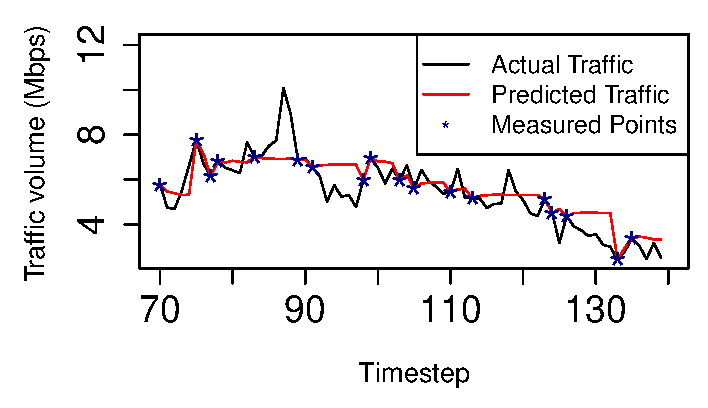
\includegraphics[width=0.28\columnwidth]{evaluation_figs/arima_flow_142_day_10.eps}  
    }
    \hfill
    \subfigure[The LSTM network
    \label{fig:prediction_result_lstm}]{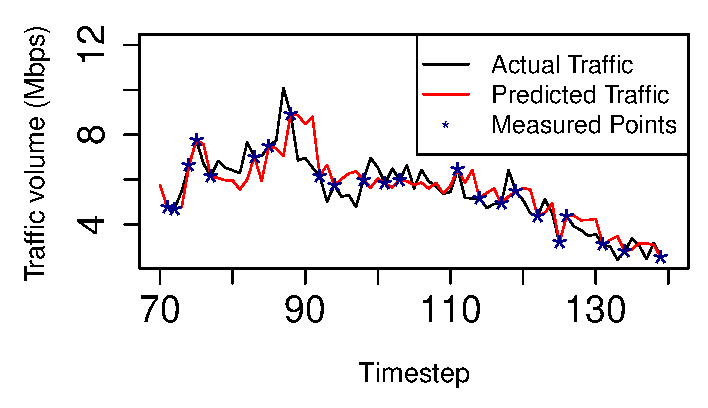
\includegraphics[width=0.28\columnwidth]{evaluation_figs/lstm_flow_142_day_10.eps}
    }
      \hfill
    \subfigure[Our proposal
    \label{fig:prediction_result_our}]{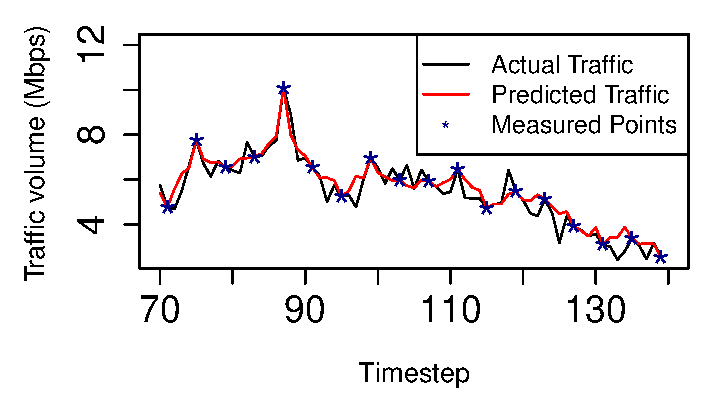
\includegraphics[width=0.28\columnwidth]{evaluation_figs/cnn_brnn_flow_11_10_day_10.eps}
    }
    \vspace{-10pt}
	\caption{Prediction results and actual values of a random flow.} 
    \label{fig:prediction_result}
\end{figure*}
\subsection{Determining the monitored flow set}
\label{subsection:flows_selection}
Our main idea is that at each timestep $t$, we calculate a weight $w_{s,d,t}$ for each flow $(s, d)$ and choose at most $k$ flows which have the lowest weights to monitor at the next timestep (i.e., timestep $t+1$). The maximum number of flows that can be monitored (i.e., $k$) depends on the network monitoring policy. In the following, before going to the details of the weight's formula, we will first describe our theoretical basis. To ease the presentation, we call the periods between the consecutive measured timesteps of a flow as non-monitored periods of that flow.

Following the experiment results shown in Section \ref{subsection:motivation}, we note that the longer the non-monitored periods, the larger the difference between the predicted results and the actual traffic. Thus, in order to reduce the prediction error, we should decrease the non-monitored periods of all flows. More specifically, the flows that have not been monitored for a long period should be chosen to be monitored at the next timestep. To this end, for each flow $(s,d)$, we define a term named \textit{consecutive missing} (denoted as $c_{s,d,t}$) which is the number of the timesteps from when $(s,d)$ was last monitored till the current timestep $t$. The weight should be designed so that it will decline when the consecutive missing gets high.

Moreover, since our imprecise data correction algorithm is based on the outputs of the forward and backward networks, we need to keep the losses of these networks (i.e., $l^f_{s,d,t}$ and $l^b_{s,d,t}$, respectively) as smaller as possible. Accordingly, the flows with higher forward and backward losses should be chosen to be monitored at the next timestep.
%since our imprecise data correction algorithm is based on the forward and backward losses (defined in Section \ref{subsection:data_correction}), the algorithm may perform well in correcting the imprecise data of flows whose losses are lower than the others. Therefore, in order to alleviate this accumulative error, the flows with high backward loss and forward loss should be chosen to be monitored at the next timestep.

Finally, we see that the flows with high fluctuation tend to have high prediction error. Therefore, these flows should be monitored more frequently. In order to measure the unsteadiness of flow $(s,d)$, we use the standard deviation of the traffic volume of the flow $(s,t)$ from timestep $t-J+1$ to $t$ (denoted as $\eta_{s,d,t}$). 

Consequently, the weight is calculated based on the flows' consecutive missing, backward loss, forward loss, and fluctuation as follows.
\begin{equation}
\label{eq_flow_weight}
\begin{aligned}
&w_{s,d,t} \\
& \ = \frac{1}{\lambda_1 \times l^f_{s,d,t} + \lambda_2 \times l^b_{s,d,t} + \lambda_3 \times c_{s,d,t} + \lambda_4 \times \eta_{s,d,t}}
\end{aligned}
\end{equation}
where $\lambda_1$, $\lambda_2$, $\lambda_3$ and $\lambda_4$ are hyper-parameters which are chosen by experiments.  

At the end of the timestep $t$, the weights of all flows are calculated, and the first $k$ flows with the lowest weights are chosen to be measured at the next timestep (i.e., timestep $t+1$).
%($d$ is the maximum number of flows can be measured depend on the network monitoring policy).
% \begin{figure}
% \RawFloats
% \begin{minipage}{0.45\textwidth}
% 	\centering
% 	\includegraphics[width=1\columnwidth]{preliminaries_figs/definitions.eps}
% 	\caption{Illustration of definitions. \label{fig:def}}
% \end{minipage}
% \hfill
% \begin{minipage}{0.45\textwidth}
% 	\centering
% 		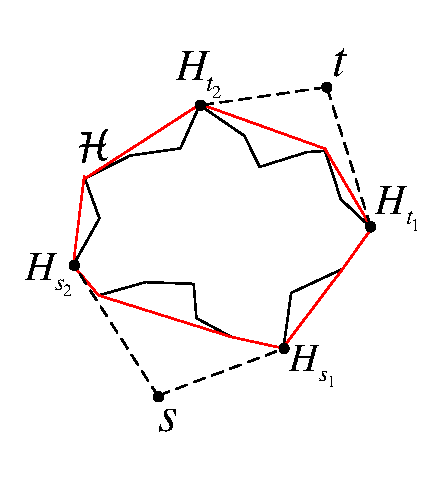
\includegraphics[width=0.8\columnwidth]{motivation_figs/shortest_path.eps}
% 		\caption{Illustration of Proposition \ref{pro:shortest_path}. \label{fig:pro_shortest_path}}
% \end{minipage}
% \end{figure}
\section{Performance evaluation}
\label{sec:performance_evaluation}
\subsection{Settings}
\begin{figure*}[bt]
  \subfigure[Error Ratio\label{fig:er_onestep}]{
  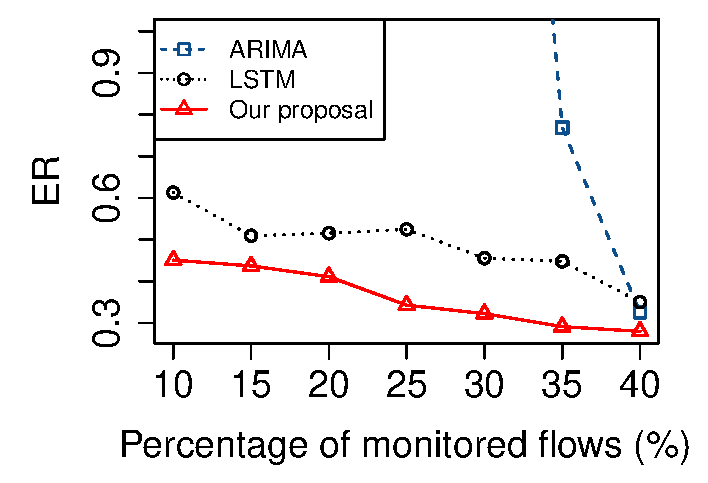
\includegraphics[width=.28\textwidth]{evaluation_figs/ER_one_step_prediciton.eps}
  }
  \subfigure[Root Mean Square Error\label{fig:rmse_onestep}]{
  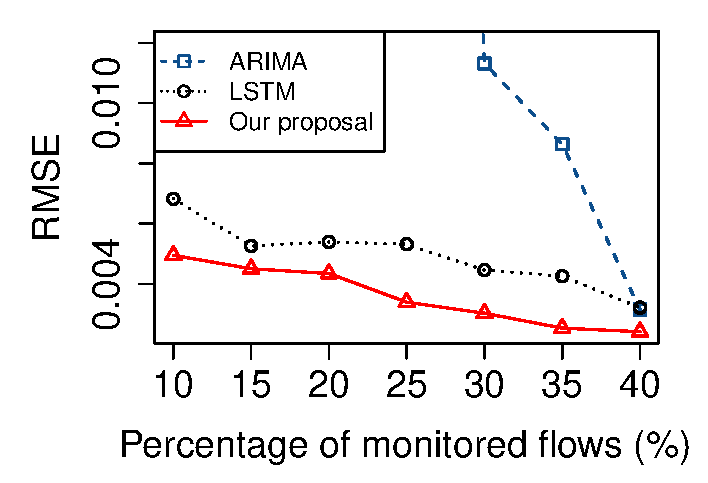
\includegraphics[width=.28\textwidth]{evaluation_figs/RMSE_one_step_prediciton.eps}
  }
  \subfigure[Coefficient of Determination\label{fig:r2_onestep}]{
  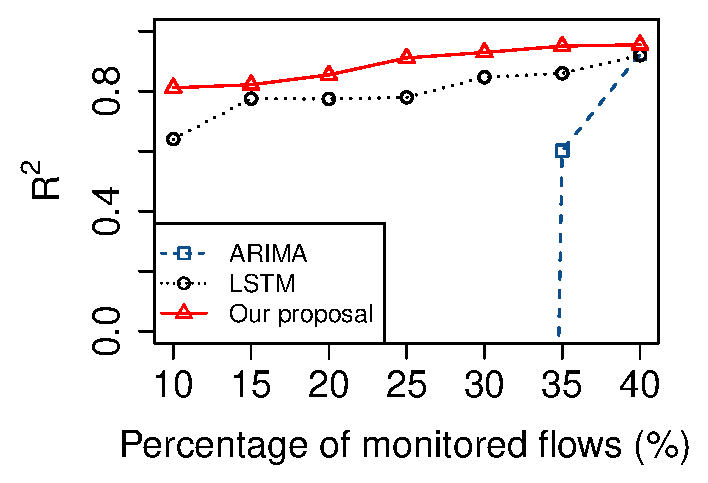
\includegraphics[width=.28\textwidth]{evaluation_figs/R2_one_step_prediciton.eps}
  }
  \vspace{-10pt}
\caption{Performance comparison in one-step-ahead prediction.}
\label{fig:result_onestep_prediction}
\end{figure*}
\begin{figure*}[bt]
  \subfigure[Error Ratio\label{fig:er_multistep}]{
  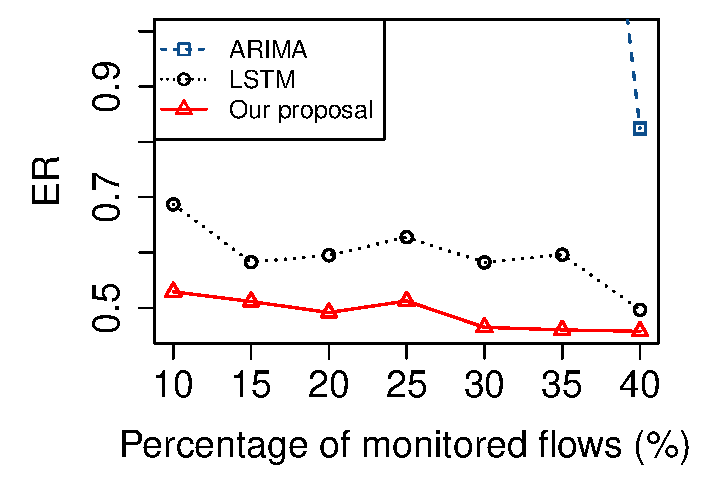
\includegraphics[width=.28\textwidth]{evaluation_figs/ER_multistep_prediciton.eps}
  }
  \subfigure[Root Mean Square Error\label{fig:rmse_multistep}]{
  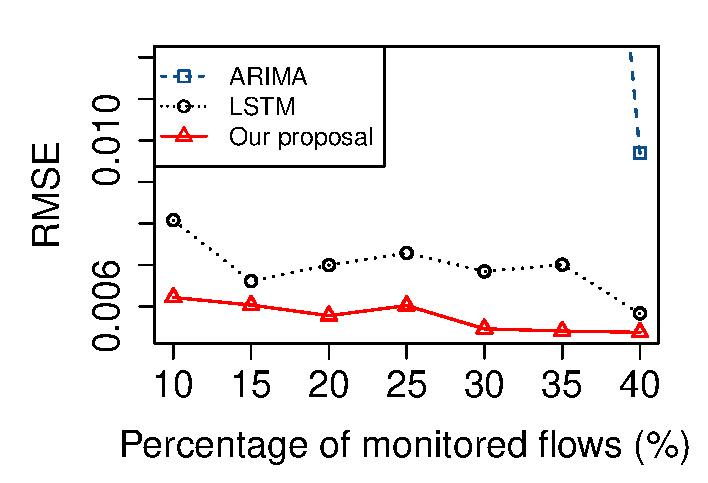
\includegraphics[width=.28\textwidth]{evaluation_figs/RMSE_multistep_prediciton.eps}
  }
  \subfigure[Coefficient of Determination\label{fig:r2_multistep}]{
  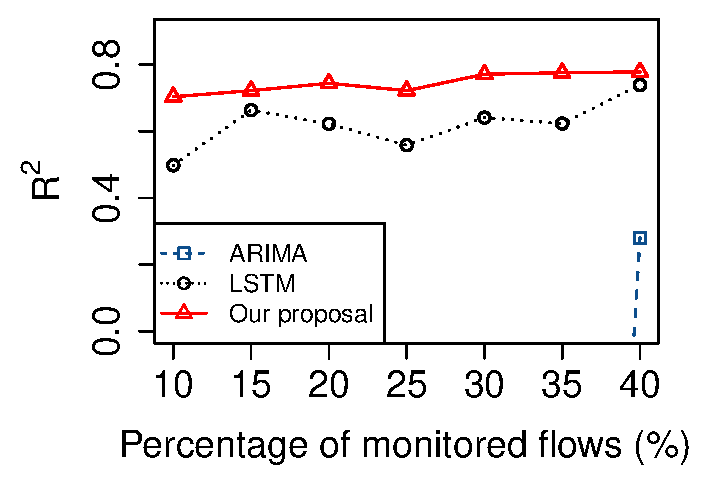
\includegraphics[width=.28\textwidth]{evaluation_figs/R2_multistep_prediciton.eps}
  }
 \vspace{-10pt}
\caption{Performance comparison in multi-step-ahead prediction.}
\label{fig:result_multistep_prediction}
%\vspace{-10pt}
\end{figure*}
\begin{table}
\caption{The configurations of ConvLSTM networks.}
\label{table:convlstm_configurations}
\resizebox{\textwidth}{!}{%
\begin{tabular}{|l|c|l|c|}
\hline
\begin{tabular}[c]{@{}l@{}}Convolutional layers\end{tabular} & 2 & Recurrent dropout & 0.2 \\ \hline
No. of filters & 8/layer & $J$ & 26 \\ \hline
Filter size & (3, 3, 2) & $L$ & 12 \\ \hline
Padding & `same' & No. of trained epoches & 50 \\ \hline
\begin{tabular}[c]{@{}l@{}}CNN dropout\end{tabular} & 0.0 & Batch size & 256 \\ \hline
\begin{tabular}[c]{@{}l@{}}$\lambda_1$, \quad $\lambda_2$\end{tabular} & \begin{tabular}[c]{@{}c@{}}2.0, \quad 1.0\end{tabular} & \begin{tabular}[c]{@{}l@{}}$\lambda_3$, \quad $\lambda_4$\end{tabular} & \begin{tabular}[c]{@{}c@{}}5.0, \quad 0.4\end{tabular} \\ \hline
\end{tabular}%
}
\vspace{-10pt}
\end{table}
We evaluated the performance of our proposed approach by conducting extensive experiments on the Abilene dataset (available at \cite{zhang2011abilene}). The dataset contains the real trace data from the backbone network located in North America which contains 12 nodes ($n = 12$). The Abilene dataset, which includes averages over 5 minutes interval of 144 origin-destination flows from March 1 to September 11, 2004, has been widely used for performance evaluation in many traffic matrix interpolation and prediction studies \cite{xie2015sequential}, \cite{xie2016accurate}. In the experiments, we separated the dataset into 60$\%$ for training, 20$\%$ and 20$\%$ for testing and validating, respectively. We compared our proposal with ARIMA \cite{box2015time} and the standard LSTM model. For ARIMA, we use the historical data of one month as the input for predict future traffic at each timestep. The performance metrics used including Error Ratio ($ER$), Root Mean Square Error ($RMSE$) and Coefficient of Determination (denoted as $R^2$ score) which are defined in (\ref{equation:metrics}). The $ER$ and $RMSE$ are used for measuring the prediction error and the standard deviation of the differences between predicted values and ground-truth values, respectively (the lower values is better). The $R^2$ score determines how well the predicted values are generated by the model. The maximum value of $R^2$ is 1 and it can be a negative number. Moreover, a higher $R^2$ is better.  
\begin{equation}
\label{equation:metrics}
\begin{aligned}
&ER = \frac{\sqrt{\sum_{s,d \in \mathcal{N}}\sum_{i=1}^T{(1-m^i_{s,d})\times(o_{s,d}^i - x_{s,d}^i)^2}}}{\sqrt{\sum_{s,d \in \mathcal{N}}\sum_{i=1}^T{(1-m^i_{s,d})\times(o^i_{s,d})^2}}} \\
&RMSE=\sqrt{\frac{1}{D}\sum_{s,d \in \mathcal{N}}\sum_{i=1}^T{(o^i_{s,d} - x^i_{s,d})^2}}\\
&R^2=1-\frac{\sum_{s,d \in \mathcal{N}}\sum_{i=1}^{T}{(o^i_{s,d}-x_{s,d}^i)^2}}{\sum_{s,d \in \mathcal{N}}\sum_{i=1}^{T}{(o^i_{s,d}-\overline{o}_{s,d}^i)^2}}
\end{aligned}
\end{equation}
where $T$ is the number of timesteps, $D = T \times n \times n$ is the size and $\overline{o}_{s,d}^i = \frac{1}{D}\sum_{s,d \in \mathcal{N}}\sum_{i=1}^{T}{o^i_{s,d}}$ is the mean of the testing dataset. 
The experiments have been conducted on a computer which has Intel i7-6900K CPU @ 3.20GHz, 48 GB memory and two NVIDIA GeForce GTX 1080Ti. The detail configurations of the ConvLSTM networks (the forward and backward networks have the same configurations) are listed in Table \ref{table:convlstm_configurations}.

We conducted two experiments. First, we evaluated the performance of all the three algorithms in one-step-ahead traffic matrix prediction ($L=1$). In the second experiment, we conducted a multi-step-ahead traffic matrix forecasting by predicting the traffic matrices of one hour ahead of the current timestep ($L = 12$). We denote $p$ as the percentage of the monitored flows per timestep. In each experiment, we conducted different scenarios in which $p$ is varied from $10\%$ to $40\%$ (i.e., the maximum number of monitored flows per timestep is $k = p \times n \times n$). 

In the following, we will show the numerical results.
Note that since the values regarding ARIMA are extremely large and lie outside the boundaries of the figures, they are also presented in Table \ref{table:arima_results}. 
%Besides that, we use Table \ref{table:arima_results} to present the results of ARIMA approach in both one-step-ahead prediction (i.e., the left value) and multi-step-ahead prediction (i.e., the right value) since the values are extremely large and lie outside the boundaries of the figures. 
\subsection{One-step-ahead traffic prediction results}
%we made the traffic prediction with different values of $k$ ($k$ is the number of monitored flows in each timestep). $k$ is equal to 10$\%$, 15$\%$, 20$\%$,...,40$\%$ of the total number of flows (i.e., $n \times n$).
In this section, we present the performance evaluation in one-step-ahead traffic prediction.
First, we evaluate how well the algorithms can capture the traffic trend (Fig.\ref{fig:prediction_result}). 
%by first show the comparison of the overall performance of all algorithm in Fig.\ref{fig:prediction_result}. 
The figure shows the difference between the predicted values and the actual values of a flow chosen randomly in about 6 hours (with 30$\%$ flows are monitored). As shown, our algorithm can capture the traffic trend much more smoothly compared with the other two algorithms. 
Besides that, thanks to the monitoring policy (described in Section \ref{subsection:flows_selection}), our proposal monitors the traffic at more spikes than ARIMA and LSTM (which use simple random policies in deciding monitored flows). 
%our proposal performs better in determining the time to monitor the flow at the spike, compared with the random policy used in ARIMA and LSTM approaches. 

Fig.\ref{fig:result_onestep_prediction} shows the performance comparison among ARIMA, LSTM and our proposed approach in terms of the Error Ratio, Root Mean Square Error and Coefficient of Determination. 
%In overall, the LSTM and ConvLSTM approaches show the superiority in modeling and predicting the temporal sequence when their results outperform the ARIMA approach in terms of all metrics. 
It can be seen that our proposal achieves the best performance regarding all the metrics. LSTM shows the second best performance and ARIMA is the worst. Comparing LSTM and our proposal, we can see that our approach achieves a high accuracy in most of the experiment scenarios. Specifically, in the best case (i.e., $p=35\%$ flows are monitored), the $ER$ and $RMSE$ of our algorithm are 35.0$\%$ and 40.5$\%$ less than that of LSTM, respectively. 
In terms of $R^2$ score, our proposal achieves 26.7$\%$ better than the LSTM approach in the best case (i.e., $p=10\%$). Moreover, it can be seen that our proposal in case $p=25\%$, achieves better performance (regarding all metrics) as LSTM in case $p=40\%$.
%our approach shows the same performance (in all metrics) while requires only 25$\%$ of ground-truth input comparing with 40$\%$ in case of using LSTM.
%(i.e., the ratio of monitored flows). 
 %Specifically, in the case of using 35$\%$ ground-truth data as input, our proposed approach results in the $ER$ and $RMSE$ that are less than 39.8$\%$ and 44.9$\%$ that of LSTM, respectively. In term of $R^2$ score, we achieve 12$\%$ better than LSTM approach.
%In addition, Fig.\ref{fig:result_onestep_prediction} indicates that while the results of our approach steadily decreases (in terms of $ER$ and $RMSE$) or increases (in terms of $R^2$ score) when increasing the ratio of the monitored flows, LSTM does not. 
%the figures of LSTM shows the dynamic in the trend. 
In addition, Fig.\ref{fig:result_onestep_prediction} indicates that while the performance of our proposal is improved gradually when increasing the number of monitored flows, LSTM does not.
The fluctuation in the results of LSTM can be explained by the random policy in choosing flows to be monitored after each timestep. 

The ratio of ground-truth input has a massive impact on the prediction accuracy of ARIMA. As shown in Table \ref{table:arima_results}, when $p < 25\%$, we see the dramatical increase of $ER$ and $RMSE$. Specifically, when $p = 10\%$, $ER$ and $RMSE$ become extremely large, i.e., $ER=2.45\mathrm{e}10$, $RMSE=3.27\mathrm{e}8$.
%from 7.27 to 2.45e10 and from 0.07 to 3.27e8 in $ER$ and $RMSE$, respectively. 
Similarly, the $R^2$ score also makes a huge decrease from $-41.23$ to $-5.27\mathrm{e}20$ when reducing $p$ from $25\%$ to $10\%$. However, when the percentage of ground-truth data in the input is sufficiently large (i.e., $p = 40\%$), ARIMA can performs very well and its performance is close to that of our algorithm. This results strongly emphasizes the advantage of our model in predicting the future traffic with only a small portion of ground-truth information.

% Please add the following required packages to your document preamble:
% \usepackage{graphicx}
\begin{table}[]
\caption{The prediction results of ARIMA}
\label{table:arima_results}
\resizebox{\textwidth}{!}{%
\begin{tabular}{|c|c|c|c|}
\hline
\begin{tabular}[c]{@{}l@{}}$p$\end{tabular} & $ER$ (exp1$|$exp2) & $RMSE$ (exp1$|$exp2)& $R^2$ (exp1$|$exp2)\\ \hline
$10\%$ & $2.45\mathrm{e}10$ $|$ $7.29\mathrm{e}10$ & $3.27\mathrm{e}8$ $|$ $1.05\mathrm{e}9$ & $-5.72\mathrm{e}20$ $|$ $-5.8\mathrm{e}21$ \\ \hline
$15\%$ & $3.5\mathrm{e}6$ $|$ $1.001\mathrm{e}7$ & $4.5\mathrm{e}4$ $|$ $1.4\mathrm{e}5$ & $-1.1\mathrm{e}13$ $|$ $-1.09\mathrm{e}14$\\ \hline
$20\%$ & $40220$ $|$ $158861$ & $323.75$ $|$ $1406$ & $-1.48\mathrm{e}9$ $|$ $-2.8\mathrm{e}10$\\ \hline
$25\%$ & $7.27$ $|$ $17.98$ & $0.07$ $|$ $0.21$ & $-41.23$ $|$ $-341.6$\\ \hline
$30\%$ & $2.89$ $|$ $11.5$ & $0.032$ $|$ $0.087$ & $-13.6$ $|$ $-148.2$ \\\hline
$35\%$ & $0.77$ $|$ $2.04$ & $0.008$ $|$ $0.03$ & $0.62$ $|$ $-3.58$ \\ \hline
$40\%$ & $0.33$ $|$ $0.83$ & $0.003$ $|$ $0.009$ & $0.92$ $|$ $0.28$\\ \hline
\end{tabular}%
}
\vspace{-10pt}
\end{table}
\subsection{Multi-step-ahead traffic prediction results}
In this section, we present the results of multi-step-ahead traffic prediction under various settings of the ratio of the monitored flows. 
In each timestep, our proposed algorithm and LSTM predict the traffic matrices of one hour ahead by applying the IMS approach, while ARIMA uses the Direct Multi-Step approach.
%In each timestep, we forecast the traffic matrices of one hour ahead by applying the IMS approach (except that ARIMA uses the Direct Multi-Step approach). 

Fig.\ref{fig:result_multistep_prediction} shows the performance evaluation of all the three algorithms in terms of $ER$, $RMSE$ and $R^2$ score.
In general, similar to the first experiment, our approach achieves the best performance in all scenarios, followed by LSTM and ARIMA. In comparison with LSTM, 
in the best case (i.e., 10$\%$ of flows are monitored), the  $ER$, $RMSE$ of our algorithm are about 23.0$\%$ less than that of LSTM. 
Moreover, our algorithm results in the $R^2$ score that is 41.2$\%$ less than LSTM.  
%our proposal decreases 0.167 (24.6$\%$), 0.00197 (24.62$\%$), and improves 0.211 (29.4$\%$) in terms of $ER$, $RMSE$, and $R^2$ score, respectively. 
Similar to the first experiment, ARIMA also shows very poor performance compared to the other two approaches. 

Comparing the results of the two experiments, it can be seen that the performance of the three algorithms in the second experiment is worse than that in the first experiment. 
However, the degradation of ARIMA is much more larger than that of our approach and LSTM. 
Specifically, in the best case (i.e., the percentage of the monitored flows is 10$\%$), the prediction errors of our approach and LSTM increase by only 17.3$\%$ and 12.5$\%$, respectively, while that of ARIMA is 197.6$\%$. 
%Considering the performance of the three algorithms in the two experiments, it can bee seen that the per
%Comparing the performance of the algorithms 
%We make the comparison between the results of the second experiment with the previous one. 
%Considering the best case, the prediction error of our approach and LSTM only increase 17.02 $\%$ and 11.14$\%$, respectively, while this value of ARIMA is 147.3$\%$. In addition, the increasings in term of $RMSE$ are 25$\%$, 18$\%$, and 184$\%$. In $R^2$ score, despite of achieving a high value (in case $p = 40\%$) in the on-step-ahead prediction, this value of ARIMA drops 70$\%$ in the second experiment. This drop of our model and LSTM are $18.5\%$ and $19.27\%$ respectively.

In summary, by applying the Convolutional LSTM network and the forward/backward data correction technique, our proposal shows the superiority in handling the missing ground-truth in the historical data.
Specifically, our proposed algorithm reduces the $ER$, $RMSE$ and increases the $R^2$ significantly compared to LSTM and ARIMA. 
%in order to achieve the high accurate traffic matrix prediction in both experiments.

% It can be seen that the performance of all algorithms in multi-step-ahead prediction is worse than that in one-step-ahead prediction. Moreover, the gap between the performance of the two experiments of our proposal and LSTM is greater than that of ARIMA. This can be explained by the use of IMS.
% %However, due to applying the IMS for multi-step prediction, the LSTM and our approach are witnessed a considerable loss in the performance evaluation in terms of all metrics. 
% For example, regarding the $ER$, while ARIMA only increases the error by y$\%$, those values of LSTM and our proposal are increased by 10$\%$ and 14.6$\%$, respectively. 
% %LSTM and our algorithm suffer the high loss in the second experiment since they use the IMS approach while the ARIMA use the Direct Multi-Step (DMS) approach for predicting multi traffic matrices. 
% Indeed, the authors in \cite{shi2018machine} have proved that DMS is more accurate than the IMS but it is difficult to train.
% \begin{table}[]
% \resizebox{\textwidth}{!}{%
% \caption{The configurations of ConvLSTM networks.}
% \label{table:convlstm_configurations}
% \begin{tabular}{|l|c|l|c|}
% \hline
% \multicolumn{4}{|c|}{ConvLSTM configurations}                                                                                                                                                    \\ \hline
% \begin{tabular}[c]{@{}l@{}}Number of \\ Convolutional \\ layer\end{tabular} & 2                        & Recurrent Dropout                                                                    & 0.0 \\ \hline
% Number of fillers                                                        & 8/layer                  & \begin{tabular}[c]{@{}l@{}}$J$ (No. of previous\\  traffic matrices)\end{tabular}      & 26  \\ \hline
% Kernel size                                                                   & (3, 3)                   & \begin{tabular}[c]{@{}l@{}}$L$ (No. of timesteps \\ in multi-step \\ prediction)\end{tabular} & 12  \\ \hline
% Padding                                                                  & 'same'                   & Training epochs                                                                      & 50  \\ \hline
% \begin{tabular}[c]{@{}l@{}}Convolutional \\ Dropout\end{tabular}                                                                  & \multicolumn{1}{c|}{0.2} & Batch size                                                                           & 256 \\ \hline
% \begin{tabular}[c]{@{}l@{}}$\lambda_1$ \\ $\lambda_2$\end{tabular}                                                                  & \multicolumn{1}{c|}{2\\1} & $\lambda_3$\\$\lambda_4$                                                                           & {5\\0.4} \\ \hline
% \end{tabular}%
% }
% \end{table}
\section{Related work}
\label{sec:related_work}
%Traffic monitoring can be classified into two main categories. The first one is traffic matrix estimation which usually estimates the missing traffic data, and the second one is traffic prediction which forecasts the future traffic. 
Traffic matrix estimation and prediction, especially in backbone networks, have attracted a lot of attention in the research community. 
To solve the traffic matrix estimation problem, the authors in \cite{hu2015cracking} exploited the compressive sensing and network tomography to recover the missing data in the traffic matrices. Moreover, the studies \cite{xie2016accurate} and \cite{xie2017accurate} considered the spatial and temporal features by proposing a new structure of the traffic matrices (3-way tensor).
%in order to estimate the missing elements in the traffic measurement data. 
The above methods can reduce the monitoring overhead by using only a small number of measurement data (under 30$\%$). However, these approaches focused on the traffic interpolation problem while many network applications and management tasks require to forecast the future traffic usage or demand.

In the traffic matrix prediction problem, originally, researchers referred to some simple statistical models such as ARIMA or Gaussian model \cite{zhou2017accurate}. However, such simple models cannot handle the complexity and dynamics of the communication behavior in modern networks. 
%to handle the complicated and dynamic in the communication behavior, 
To this end, deep learning techniques have been exploited more in predicting traffic \cite{wang2017spatiotemporal, cao2018interactive, nie2016traffic}. 
In \cite{wang2017spatiotemporal} and \cite{cao2018interactive}, the authors utilized the Long Short-Term Memory and Convolutional Neural Network for capturing the spatiotemporal feature and predicting the network traffic in data center and cellular networks, respectively. In backbone network, Nie et al. \cite{nie2016traffic} used Restricted Boltzmann Machine to capture the dynamic features of network. The authors then proposed two separated deep belief network models for solving the traffic estimation and prediction, independently. More recent, the results in \cite{azzouni2018neutm} and \cite{vinayakumar2017applying} showed the superiority of LSTM network in modeling the temporal feature and the long-range dependencies of network traffic. Unfortunately, all the approaches proposed so far assumed that the input contains only the ground-truth data. To the best of our knowledge, there is no existing work addressing the problem of traffic prediction under missing ground-truth data in backbone network.

\section{Conclusion}
\label{sec:conclusion}
In this paper, we addressed the traffic matrix prediction problem in backbone networks where the future traffic is estimated under the lack of precise historical data. We exploited the Convolutional LSTM network for extracting and modeling the spatiotemporal feature of the traffic matrices. We proposed a novel deep learning model and techniques which leverage the forward and backward ConvLSTM networks to correct input data and determine flows monitored at the next timestep. We conducted extensive experiments for evaluating our proposed approach. The results demonstrated that the proposed approach outperforms other well-known methods for time series analysis. 


%\section*{Acknowledgment} 
%This research is supported in part by 
\newcommand{\BIBdecl}{\setlength{\itemsep}{0.25 em}}
\bibliographystyle{unsrt}
\bibliography{im}
% \appendix
% \label{sec:appendix}
% \begin{myproof}[of Proposition \ref{pro:scale_factor}] 
\label{proof:scale_factor}
\normalfont
In the following, we prove a more general statement: Let $\mathcal{Q}$ be a convex polygon, and let $\mathcal{P}$ be another convex polygon that entirely covers $\mathcal{Q}$. Then, for any two arbitrary points $s$ and $t$ outside of $\mathcal{P}$, we have
\begin{equation}
\label{statement}
\nonumber 
\left|  L_\mathcal{P}(s,t) \right |  \leq  \left|  L_\mathcal{Q}(s,t) \right |  +  p_\mathcal{P} - p_\mathcal{Q} (*)
\end{equation}
Figure \ref{fig:pro_1} illustrates the proof.
%\noindent \textbf{Proof (of Proposition \ref{lem:lemma1}).}\\
Let $Q_1, ..., Q_n$ denote the vertices of $\mathcal{Q}$, and let $P_1, ..., P_m$ denote the vertices of $\mathcal{P}$, which are ordered in the counterclockwise direction.
Let $s{ \{Q_u \sim Q_{u+k} \}}^{+}_\mathcal{Q} t$ denote the shortest path between $s$ and $t$ that bypasses $\mathcal{Q}$, and assume that this path stays on the right side of $\overrightarrow{st}$.
According to Proposition \ref{pro:shortest_path}, $Q_u$ and $Q_{u+k}$ must be view-limit vertices of $\mathcal{Q}$ with respect to $s$ and $t$, respectively.
%\begin{figure}[bt]
%	\centering
%	\includegraphics[width =0.35\columnwidth]{strategy_4.eps}
%	\vspace{-8pt}
%	\caption{Illustration of the proof of Theorem \ref{lem:strategy_4}.\label{fig:strategy_4}}
%\end{figure}
Let $P_v, .., P_{v+h}$ denote all vertices of $\mathcal{P}$ that are on the right side of $\overrightarrow{st}$; then, $L_\mathcal{P}(s,t) \leq s{ \{ P_v \sim P_{v+h} \} }^{+}_\mathcal{P}t$. 
Let $Q^{'}_{u}$ and $Q^{'}_{u+k}$ denote the intersections of $sQ_u$ and $tQ_{u+k}$ with $P_{v-1}P_v$ and $P_{v+h}P_{v+h+1}$, respectively. Then,  
\begin{footnotesize}
\begin{equation}
\label{eq:n_4_1}
L_\mathcal{P}(s,t)  \leq s{ \{ P_v \sim P_{v+h} \} }^{+}_\mathcal{P}t 
 \leq \left |sQ^{'}_{u} \right | + \left | { \{ Q^{'}_{u} \sim Q^{'}_{u+k}\} }^{+}_\mathcal{P} \right | + \left |Q^{'}_{u+k}t \right |  
\end{equation}
\end{footnotesize}
%\begin{equation}
%\begin{split}
%\label{eq:n_4_1}
%l_\mathcal{P}(s,t) & \leq s{ \{ P_v \sim P_{v+h} \} }_\mathcal{P}t \\
%& \leq \left |sQ^{'}_{u} \right | + \left | { \{ Q^{'}_{u} \sim Q^{'}_{u+k}\} }_\mathcal{P} \right | + \left |Q^{'}_{u+k}t \right |  
%\end{split}
%\end{equation}
It is obvious that
\begin{footnotesize}
\begin{equation}
\label{eq:n_4_2}
\left | Q_{u+k} Q^{'}_{u+k} \right | + \left | { \{ Q^{'}_{u+k} \sim Q^{'}_{u} \} }^{+}_\mathcal{P}\right | + \left | Q^{'}_{u}Q_u\right | \geq \left | {\{ Q_{u+k} \sim Q_u \}}^{+}_\mathcal{Q}\right |  
\end{equation}
\end{footnotesize}
Note that $p_\mathcal{P}= \left | { \{ Q^{'}_{u} \sim Q^{'}_{u+k} \} }^{+}_\mathcal{P}\right | +  \left | { \{ Q^{'}_{u+k} \sim Q^{'}_{u} \} }^{+}_\mathcal{P}\right | $.
Therefore, from (\ref{eq:n_4_2}), it can be deduced that
\begin{footnotesize}
\begin{equation}
\label{eq:n_4_3}
\left | { \{ Q^{'}_{u} \sim Q^{'}_{u+k} \} }^{+}_\mathcal{P}\right | \leq p_\mathcal{P} -  \left | {\{ Q_{u+k} \sim Q_u \}}^{+}_\mathcal{Q}\right |  
+ \left | Q_{u+k} Q^{'}_{u+k} \right | +  \left | Q^{'}_{u}Q_u\right | 
\end{equation}
\end{footnotesize}
%\begin{equation}
%\begin{split}
%\label{eq:n_4_3}
%\left | { \{ Q^{'}_{u} \sim Q^{'}_{u+k} \} }_\mathcal{P}\right | \leq p_\mathcal{P} &-  \left | {\{ Q_{u+k} \sim Q_u \}}_\mathcal{Q}\right |  \\
%&+ \left | Q_{u+k} Q^{'}_{u+k} \right | +  \left | Q^{'}_{u}Q_u\right | 
%\end{split}
%\end{equation}
Note that $p_\mathcal{Q}= \left | { \{ Q_{u} \sim Q_{u+k} \} }^{+}_\mathcal{Q}\right | +  \left | { \{ Q_{u+k} \sim Q_{u} \} }^{+}_\mathcal{Q}\right | $.\\
Therefore, (\ref{eq:n_4_3}) is equivalent to
\begin{equation}
\begin{split}
\label{eq:n_4_4}
\left | { \{ Q^{'}_{u} \sim Q^{'}_{u+k} \} }^{+}_\mathcal{P}\right | \leq p_\mathcal{P} - p_\mathcal{Q}  & +  \left | { \{ Q_{u} \sim Q_{u+k} \} }^{+}_\mathcal{Q}\right |  \\
& + \left | Q_{u+k} Q^{'}_{u+k} \right | +  \left | Q^{'}_{u}Q_u\right | 
\end{split}
\end{equation}
By adding (\ref{eq:n_4_1}) and (\ref{eq:n_4_4}), we obtain
\begin{equation}
\nonumber L_\mathcal{P}(s,t) \leq   L_\mathcal{Q}(s,t) + p_\mathcal{P} - p_\mathcal{Q}
\end{equation}
Thus, Statement (*) is proven. Proposition \ref{pro:scale_factor} can be directly deduced from Statement (\ref{statement}) as follows.
Because $\mathcal{F}$ is an image of $\mathcal{H}$ obtained through a homothetic transformation with a scale factor of $\xi$, $p_{\mathcal{F}} = (1-\xi)p_{\mathcal{H}}$.
Therefore, $L_\mathcal{F}(s,t) \leq  L_\mathcal{H}(s,t) + p_\mathcal{F} - p_\mathcal{H} = L_\mathcal{H}(s,t) + (\xi-1)p_\mathcal{H}$.
\end{myproof} 
\begin{figure}[hbt]
	\centering
	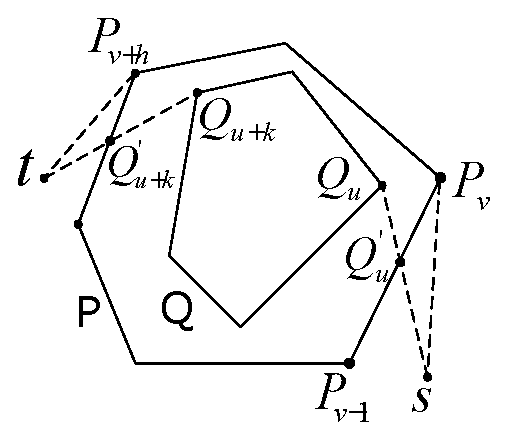
\includegraphics[width =0.35\columnwidth]{./appendix/proof_1.eps}
	\caption{Illustration of the proof of  Proposition \ref{pro:scale_factor}.\label{fig:pro_1}}
\end{figure}

%%%%%%%%%%%%%%%%%%%%%%%%%%%%%%%%%%
\IEEEpeerreviewmaketitle
\end{document}


